\chapter[FUNDAMENTAÇÃO TEÓRICA]{\textbf {FUNDAMENTAÇÃO TEÓRICA}}

\section{ANÁLISE DE MARCHA}
\section{MÉTODOS ÁGEIS}
A muito tempo vários métodos para desenvolvimento de software são propostos. 
Em 2001, um grupo de pessoas muito experientes em desenvolvimento de software, juntaram-se em Salt Lake City,Utah, para resolverem problemas de desenvolvimento de software \cite{Greene2014}.
Como resultado deste encontro, foi criado o manifesto ágil, que é reproduzido a seguir \cite{Beck2001}:

\begin{citacao}

Estamos descobrindo maneiras melhores de desenvolver software, fazendo-o nós mesmos e ajudando outros a fazerem o mesmo. 
Através deste trabalho, passamos a valorizar:

Indivíduos e interações mais que processos e ferramentas;

Software em funcionamento mais que documentação abrangente;

Colaboração com o cliente mais que negociação de contratos;

Responder a mudanças mais que seguir um plano.

Ou seja, mesmo havendo valor nos itens à direita, valorizamos mais os itens à esquerda.
\end{citacao}

Meses após a criação do manifesto, estas pessoas também criaram os princípios ágeis e a Aliança Ágil \cite{Layton2012}.

Os princípios ágeis são um conjunto de 12 itens com o objetivo de auxiliar na implantação de metodologias ágeis. Eles são reproduzidos a seguir a título de ilustração \cite{Beck2001}:

\begin{citacao}
		1. Nossa maior prioridade é satisfazer o cliente
		através da entrega contínua e adiantada
		de software com valor agregado.

		2. Mudanças nos requisitos são bem-vindas,
		mesmo tardiamente no desenvolvimento.
		Processos ágeis tiram vantagem das
		mudanças visando vantagem competitiva para o cliente.

		3. Entregar frequentemente software funcionando,
		de poucas semanas a poucos meses,
		com preferência à menor escala de tempo.

		4. Pessoas de negócio e desenvolvedores devem trabalhar
		diariamente em conjunto por todo o projeto.

		5. Construa projetos em torno de indivíduos motivados.
		Dê a eles o ambiente e o suporte necessário
		e confie neles para fazer o trabalho.

		6. O método mais eficiente e eficaz de transmitir
		informações para e entre uma equipe de desenvolvimento
		é através de conversa face a face.

		7. Software funcionando é a medida primária de progresso.

		8. Os processos ágeis promovem desenvolvimento
		sustentável. Os patrocinadores, desenvolvedores e
		usuários devem ser capazes de manter um ritmo
		constante indefinidamente.

		9. Contínua atenção à excelência técnica e bom design
		aumenta a agilidade.

		10. Simplicidade--a arte de maximizar a quantidade de
		trabalho não realizado--é essencial.

		11. As melhores arquiteturas, requisitos e designs
		emergem de equipes auto-organizáveis.

		12. Em intervalos regulares, a equipe reflete sobre como
		se tornar mais eficaz e então refina e ajusta seu
		comportamento de acordo. 
\end{citacao}



Este manifesto, serviu de marco agregador de métodos e técnicas, que já existiam a época, mas não eram amplamente difundidas como \emph{Scrum}, \emph{Extreme Programming}, \emph{kanban}, \emph{lean}, entre outros. 
Estas técnicas, apesar de anteriores ao manifesto, possuem em seus cernes, muito em comum com os valores ágeis.
A figura \ref{cap2_valores} tenta ilustrar esta ideia.
\begin{figure}[ht]
	\centering
	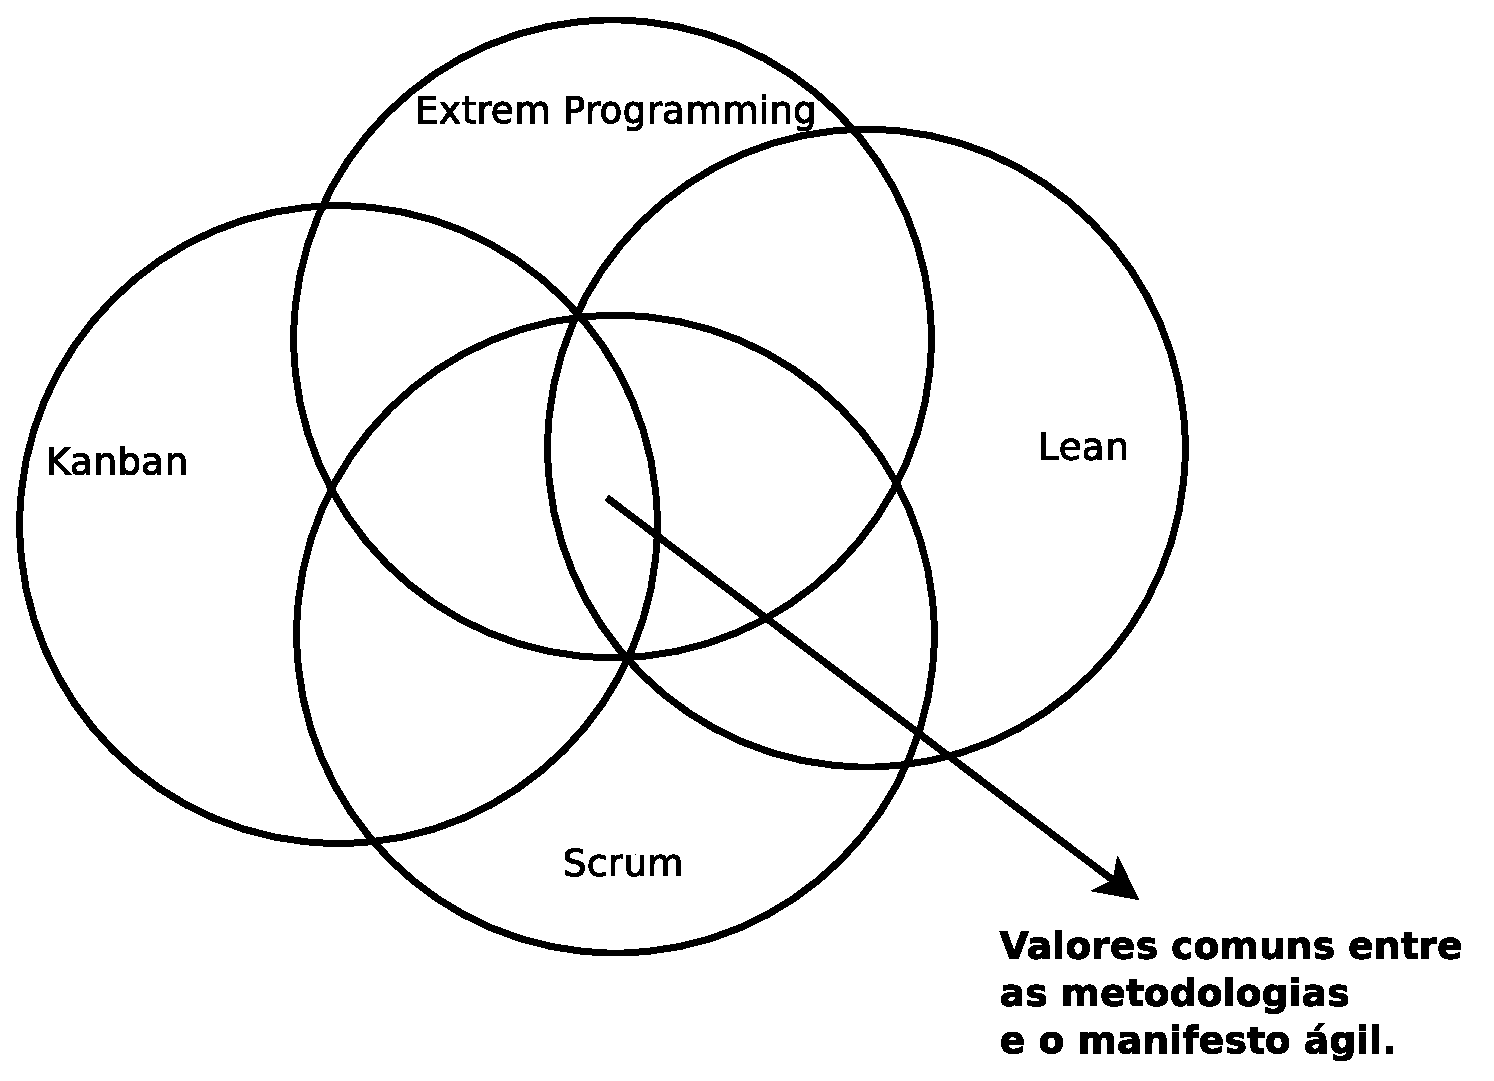
\includegraphics[width=7cm]{figuras/cap2_valores.eps}
	\caption{Valores em comum. Adaptado de \cite{Greene2014}.}
	\label{cap2_valores}
\end{figure}

A adoção dos métodos ágeis hoje é praticamente unanimidade. Isto se deve aos modelos de desenvolvimento adotados até a década de 1990. Esses modelos eram na sua grande maioria baseados no modelo \emph{waterfall}, que imitava uma linha de produção onde o software era desenvolvido em fases. A saída de cada fase era a entrada da próxima. A figura \ref{waterfall}, mostra um exemplo de processo baseado no modelo \emph{waterfall}.
\begin{figure}[ht]
	\centering
	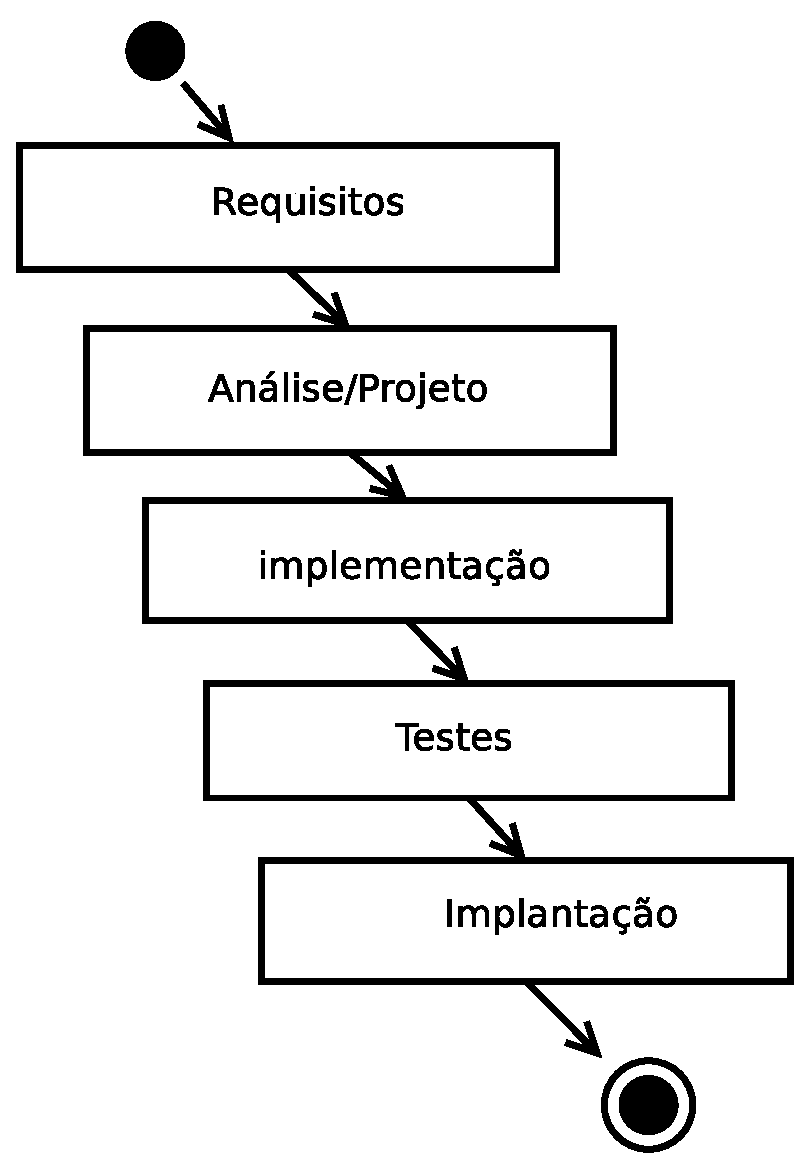
\includegraphics[width=4cm]{figuras/waterfall.eps}
	\caption{Exemplo de processo baseado no modelo \emph{waterfall}}
	\label{waterfall}
\end{figure}

O maior problema do modelo \emph{waterfall}, era que este era completamente averso a mudanças de requisitos. 
Hoje é notório que a grande maioria dos softwares necessitam ser bastante receptivos a mudanças.

\cite{KristinRunyan2014} compara o modelo \emph{waterfall} como o modelo ágil.

\begin{table}
	\caption{Comparando Modelos de Desenvolvimento de Software}
	\ABNTEXfontereduzida
	\begin{tabular}{p{8cm}p{8cm}}
	\toprule
	\textit{Waterfall} & \textit{Ágil}\\
	\midrule
	\ABNTEXfontereduzida
	Prescritivo & Abstrato\\
	Documentação extensiva & Mínimo de documentação\\
	Sequencial & Contínuo\\
	Formal & Informal\\
	Foco no processo & Foco na comunicação\\
	Mudança gradual & Mudança rápida\\
	\bottomrule
	\end{tabular}
	\footnotesize Fonte:
	\cite{KristinRunyan2014}
\end{table}


Como evolução do modelo \emph{waterfall}, surgiram os processos baseados em modelos iterativos. 
A diferença agora, é que o processo de desenvolvimento passa a ser baseado em ciclos. 
Cada ciclo passa por cada uma das fases do \emph{waterfall}. 
Este tipo de processo, apresentava melhoras, mas ainda era concebido sob a forma de um processo que visava resolver problemas determinísticos, como o das linhas de produção das fábricas.
Mas, como descrito em \cite{Beck2004}, o processo de se construir software é mais parecido com o ato de dirigir.
O motorista sabe o destino a que quer chegar, porém, durante o percurso pode haver um acidente e tem-se que mudar um pouco a rota, ou alguém está passando por uma faixa de pedestre e necessita-se parar, ou ainda um sinal de transito pode ficar vermelho. 
Esta é a principal motivação para que este trabalho, privilegie métodos ágeis de desenvolvimento.

\subsection{Scrum}

\section{SOFTWARE COMO SERVIÇO}
\section{SOFTWARE LIVRE} 
\section{APRENDIZADO DE MÁQUINA}

\goodbreak
\newpage
\clearpage

\section[CMAC]{CMAC}
\label{cmac_sec}

A \emph{Cerebellar Model Articulation Controller} (CMAC) foi criada por James Sacra Albus \cite{Albus1975b}. 
Ele se inspirou no cerebelo dos mamíferos para criá-la. 
O mesmo autor havia feito um extenso trabalho sobre o funcionamento do cerebelo \cite{Albus1971b}.
Trabalho este, que resultou numa tese de doutorado \cite{Albus1972a}.
Aplicações da CMAC podem ser vistas em \cite{Albus1975d}, \cite{Albus1979}, \cite{Sabourin2006a} e \cite{Lin2002a}.
Uma aplicação que começou a ser desenvolvida pela UnB é descrita em \citeonline{Andrade2014}. Inclusive a implementação da \emph{CMAC} desenvolvida neste trabalho teve origem nele.

Na Figura \ref{fig1} é possível ver o funcionamento básico da CMAC. Os sinais $S$ entram no sistema, que mapeiam o mesmo para um conjunto de pesos $W^*$ que devem ser somados para ativação. 
Note que apenas uma pequena fração de pesos é realmente selecionada para participar na ativação. 
O conjunto de pesos disponíveis na CMAC é necessariamente maior que o número de pesos ativados $W^*$. 

\begin{figure}[H]
	\centering
	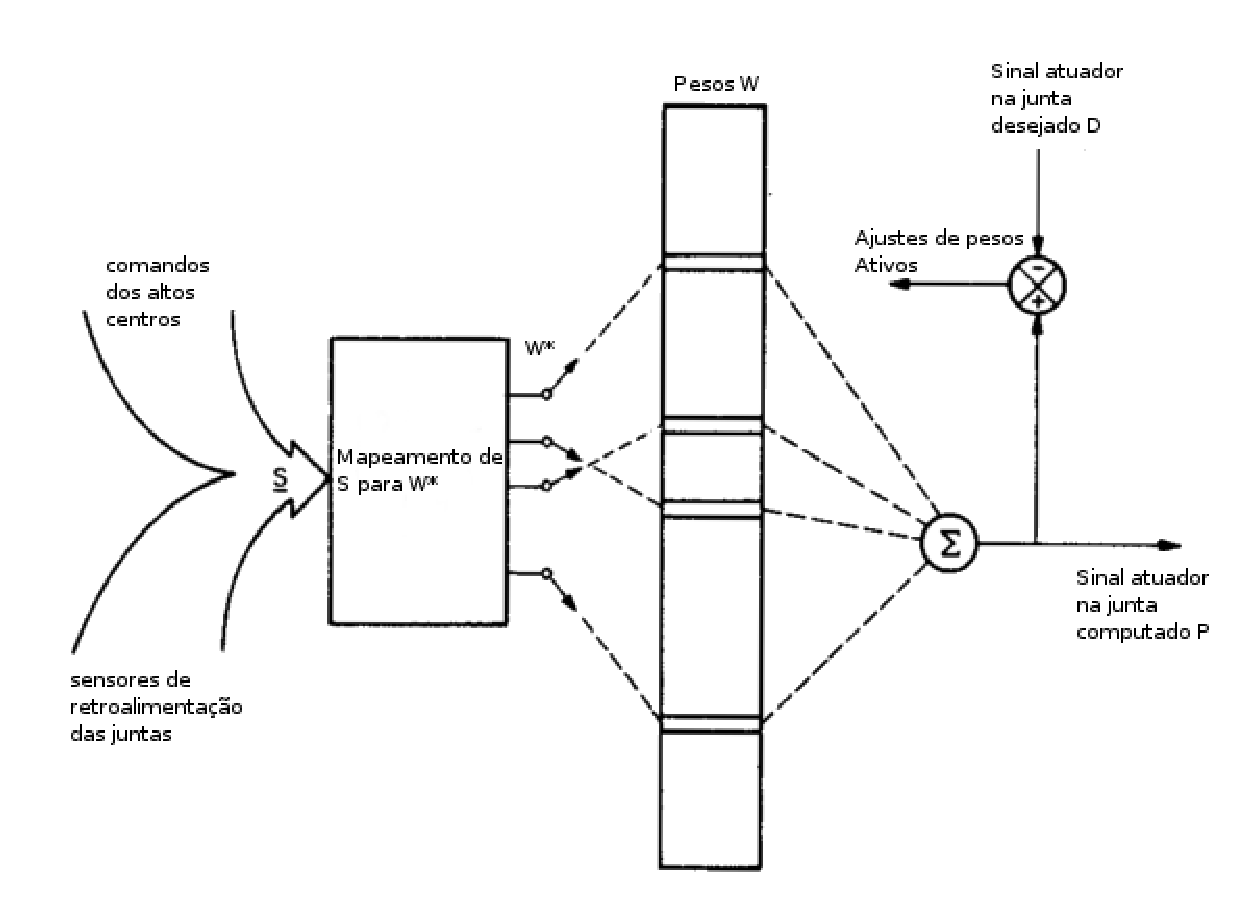
\includegraphics[width=15 cm]{figuras/cmac1.eps}
	\caption{CMAC para controle de uma junta. Fonte: (Alterado de \citeonline{Albus1975b}).}
    	\label{fig1}
\end{figure}


A CMAC da Figura \ref{fig1} também pode ser classificada como um sistema \emph{Multiple Input Single Output} (MISO), ou seja, suporta a entrada de vários sinais de entrada e processa um sinal de saída.
Para se produzir uma CMAC \emph{Multiple Input Multiple Output} MIMO, bastaria implementar várias MISOs, compartilhando as mesmas entradas.


Os passos para que o sinal seja computado são descritos a seguir. Estes passos são os mesmos descritos em \citeonline{Albus1975b}.

Primeiramente, define-se o número de pesos $NW*$ a serem ativados para comporem a saída da CMAC.

O segundo passo é quantizar os possíveis valores para cada item do vetor de entrada $S$.
Por exemplo, se o primeiro item $s1$ de $S$ aceita valores de -1 até 1 e se quer 5 valores possíveis, quantiza-se então os valores de -1 até 1, conforme a Figura \ref{inputs1}.


\begin{figure}[ht]
	\centering
	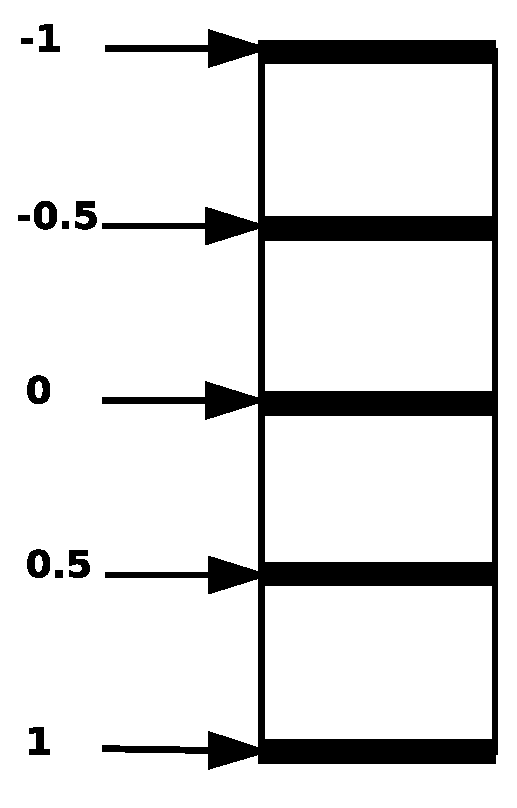
\includegraphics[width=3 cm]{figuras/input.eps}
	\caption{Quantização de $s1$.}
    	\label{inputs1}
\end{figure}


Isto significa que quaisquer que sejam os valores de $s1$ os mesmos devem ser convertidos para -1, -0,5, 0, 0,5 e 1. 
Por exemplo, se o valor de $s1$ for 0,75, será convertido para o valor 1, se for -0,75 será o valor 0 e se for 0,25 será o valor 0,5. A esta quantização dá-se o nome de resolução da CMAC \cite{Albus1975b}.

O próximo passo é criar uma tabela para cada um dos sinais discretizados de entrada do vetor $S$. 
Supondo que o vetor $S$ possui 2 sinais de entrada $s1$ e $s2$ e um número de ativações $NW*$ igual a 3, deve-se criar duas tabelas, uma para cada sinal, conforme se apresentam na Tabela \ref{disc_s1} e na Tabela \ref{disc_s2}. 
Para facilitar o entendimento, irá se considerar os valores possíveis de $s1$ iguais aos inteiros de 1 até 6 e os valores possíveis de $s2$ iguais aos inteiros de 1 até 4.
Cria-se uma coluna com os valores do sinal em questão. 
Para cada valor, cria-se 3 ($NW*$) valores novos. 
Para o primeiro valor do sinal, usa-se os 3 primeiros inteiros não negativos.
Para o segundo valor do sinal, substitui-se o primeiro dos três itens pelo próximo número após o terceiro item do sinal anterior. 
Para o terceiro sinal, substitui-se o segundo dos três itens pelo próximo inteiro não negativo.
Assim, sucessivamente conforme a Tabela \ref{disc_s1} e Tabela \ref{disc_s2} \cite{Albus1975b}.

\begin{table}[H]
	\centering
	\caption{Mapeamento de $s1$}
	\label{disc_s1}
	\ABNTEXfontereduzida
	\begin{tabular}{c c}
		\toprule
		\textit{Valore de $s1$} & \textit{Mapeamento $m1$}\\
		\midrule
		\ABNTEXfontereduzida
		1 & 0, 1, 2 \\
		2 & 3, 1, 2 \\
		3 & 3, 4, 2 \\
		4 & 3, 4, 5 \\
		5 & 6, 4, 5 \\
		6 & 6, 7, 5 \\
		\bottomrule
	\end{tabular}
\end{table}
\begin{table}[H]
	\centering
	\caption{Mapeamento de $s2$}
	\label{disc_s2}
	\ABNTEXfontereduzida
	\begin{tabular}{c c}
		\toprule
		\textit{Valore de $s2$} & \textit{Mapeamento $m2$}\\
		\midrule
		\ABNTEXfontereduzida
		1 & 0, 1, 2 \\
		2 & 3, 1, 2 \\
		3 & 3, 4, 2 \\
		4 & 3, 4, 5 \\
		\bottomrule
	\end{tabular}
\end{table}


Depois de mapeado cada valor de cada item de entrada, deve-se combinar os mapeamentos de acordo com a Tabela \ref{wmap}.

\begin{table}[ht]
	\centering
	\caption{Mapeamento para os pesos $W$}
	\label{wmap}
	\ABNTEXfontereduzida
	\begin{tabular}{c c c c c}
		\toprule
		\textit{$s1$ / $s2$} & \textit{1}  & \textit{2} & \textit{3} & \textit{4} \\
		\midrule
		\ABNTEXfontereduzida

		\textit{1} & (0, 0), (1, 1), (2, 2) & (0, 3), (1, 1), (2, 2) & (0, 3), (1, 4), (2, 2) & (0, 3), (1, 4), (2, 5) \\
		\textit{2} & (3, 0), (1, 1), (2, 2) & (3, 3), (1, 1), (2, 2) & (3, 3), (1, 4), (2, 2) & (3, 3), (1, 4), (2, 5) \\
		\textit{3} & (3, 0), (4, 1), (2, 2) & (3, 3), (4, 1), (2, 2) & (3, 3), (4, 4), (2, 2) & (3, 3), (4, 4), (2, 5) \\
		\textit{4} & (3, 0), (4, 1), (5, 2) & (3, 3), (4, 1), (5, 2) & (3, 3), (4, 4), (5, 2) & (3, 3), (4, 4), (5, 5) \\
		\textit{5} & (6, 0), (4, 1), (5, 2) & (6, 3), (4, 1), (5, 2) & (6, 3), (4, 4), (5, 2) & (6, 3), (4, 4), (5, 5) \\
		\textit{6} & (6, 0), (7, 1), (5, 2) & (6, 3), (7, 1), (5, 2) & (6, 3), (7, 4), (5, 2) & (6, 3), (7, 4), (5, 5) \\

		\bottomrule
	\end{tabular}
\end{table}
 


O mapeamento da Tabela \ref{wmap} é feito da seguinte forma \cite{Albus1975b}: 
Coloca-se cada valor quantizado de $s1$ nomeando cada uma das linhas da tabela. 
Coloca-se cada valor discretizado de $s2$ nomeando cada uma das colunas das tabelas. 
Cada célula da tabela é obtida recuperando-se os itens de $s1$ e de $s2$, que estão na Tabela \ref{disc_s1} e na Tabela \ref{disc_s2}, e concatenando-se cada item de acordo com sua posição. 
Por exemplo, para o valor de $s1$ igual a 5, recuperam-se os itens (6, 4, 5), para o valor de $s2$ igual a 2, recuperam-se os itens (3, 1, 2). 
Agora é só criar novos itens, na mesma quantidade do valor $NW*$, concatenando-se cada item de acordo com sua posição. O lista resultante é ((6, 3), (4, 1), (5, 2)). 

Cada vetor de 2 posições da Tabela \ref{wmap}, por exemplo (0, 0), (4, 1), é um rótulo de uma entrada na tabela de pesos $W$.

Para se calcular a saída do sistema, suponha que os valores de $s1$ e $s2$, ainda sejam 5 e 2, respectivamente, e $NW*$ ainda seja 3. 
Neste caso, recupera-se o item da linha 5 e da coluna 2, que é ((6, 3), (4, 1), (5, 2)). 
Agora é acessada a tabela de pesos W e são recuperados os pesos cujas chaves são (6, 3), (4, 1) e (5, 2). 
Note-se que serão recuperados exatamente 3 pesos, que é exatamente o número de ativações $NW*$ desejadas. 
Os valores recuperados constituem um vetor chamado $W*$. A saída é calculada somando-se os valores de W*.



\subsection{TREINAMENTO DA CMAC}
Sendo a CMAC uma Rede Neural Artificial (RNA) com aprendizado supervisionado, seus pesos podem ser atualizados simplesmente computando-se o erro e atualizando-se apenas os pesos que participaram do computo do sinal $P$ \cite{Haykin1998}. O processo é detalhado nos próximos parágrafos.

Para se treinar a CMAC, primeiro define-se o conjunto de dados para treinamento que devem ser usados. 
Pode ser usado algo entre 20\% e 50\% dos dados coletados para desenvolvimento do sistema. 
Cada item destes dados deve conter um vetor de sinais de entradas $S$ e a resposta desejada $D$ para estes sinais. 
A tabela de pesos deve ser inicializada com valores randômicos. 
Para cada vetor $S$ deve ser calculado o vetor $W*$, que contém os endereços dos pesos a serem ativados. 
Calcula-se, então, a saída da rede $P$ para o vetor $S$, conforme definido no item \ref{cmac_sec}, somando os itens do vetor $W$. 
Atualizam-se os pesos sinápticos conforme a Equação \ref{write_weight} adaptada de \citeonline{Sabourin2012a}.
\begin{equation}
	\label{write_weight}
	w_{i} = w_{i} + \cfrac{\alpha (D - P)}{NW^{*}}
\end{equation}

A variável $w_{i}$ é um item qualquer dentro da tabela de pesos $W$. 
Em cada iteração no conjunto de dados para treinamento, deve-se atualizar apenas os pesos descritos em $W*$ naquele momento. 
A variável $\alpha$ é o coeficiente de aprendizado, deve ser um valor entre 0 e 1. 
A variável $NW*$ é o número de valores a serem utilizados para ativação, que consequentemente equivale ao número de itens do vetor $W*$.

Deve-se determinar o número de iterações \emph{batch} para o sistema. 
Uma iteração \emph{batch} consiste no processamento dos pesos para cada item dentro do conjunto de dados para treinamento \cite{Ng2015}. 
O sistema deve continuar iterando até atingir o número de iterações \emph{batch}.

Apesar do número de iterações \emph{batch} ser válido como critério de parada para o treinamento da CMAC, nada impede o uso de outros critérios, por exemplo, o erro quadrado médio da saída $Y$ em relação ao desejado $D$.


\begin{comment}
\section[PRÓTESES TRANSFEMURAIS ATIVAS]{PRÓTESES TRANSFEMURAIS ATIVAS}

\subsection[Tipos de próteses]{\textbf{Tipos de próteses}}

As próteses constituem uma importante contribuição da engenharia na área da reabilitação humana. Existem próteses para substituição da função de membros exteriores como braços e pernas, até a substituição de secções de esôfagos ou intestinos.

As próteses para substituir as funções das pernas, em especial, têm evoluído bastante ao longo do tempo.
Existem próteses ativas e passivas para este fim. Próteses passivas são constituídas intrinsecamente por elementos mecânicos que não possuem qualquer tipo de suporte energético externo.
Já próteses ativas, são constituídas por elementos mecânicos e eletrônicos, sendo que partes mecânicas da prótese recebem auxílio de energia externa para atuar na função que está sendo substituída, por exemplo, a flexão de um joelho.
A principal vantagem das próteses ativas, sobre as passivas, está na compensação do débito energético que ocorre nas passivas. Esta compensação garante um ciclo de marcha mais confortável, suave e natural ao usuário da prótese ativa \cite{Borjian2008}.

\subsection[Projeto de controle para próteses transfemurais ativas]{\textbf{Projeto de controle para próteses transfemurais ativas}}

Em \citeonline{Sup2008}, demonstra-se o projeto de uma prótese transfemural ativas.
Este trabalho escolheu técnicas de engenharia de controle para controle da prótese.
Basicamente foram criados modelos matemáticos baseados na física clássica para, então, derivar uma equação de transferência que servirá de base para as leis de controle que atuarão na prótese. 

Em \citeonline{Vallery2011} é apresentado um enfoque novo para controle de próteses transfemurais ativas.
Este modelo é baseado em regressões estatísticas, que aplicam os sinais de entrada em um modelo estatístico para então produzir um sinal de saída.
Este é um modelo que pode ser considerado adaptativo.

O terceiro modelo encontrado de projeto de controle para próteses transfemurais ativas, foi o de \citeonline{Borjian2008}. Ele utilizou um controlador \emph{fuzzy}, especificamente com o modelo Takagi-Sygeno-Kang (TSK) \emph{fuzzy}. Este é um modelo adaptativo.




\end{comment}
